% ------------------------------------------------------------------------------
% TYPO3 CMS 6.2 LTS - What's New - Chapter "Responsive Images" (Spanish Version)
%
% @author	Sergio Catalá <sergio.catala@e-net.info>
% @author	Michel Mix <mmix@autistici.org>
% @license	Creative Commons BY-NC-SA 3.0
% @link		http://typo3.org/download/release-notes/whats-new/
% @language	Spanish
% ------------------------------------------------------------------------------
% Chapter: Responsive Images
% ------------------------------------------------------------------------------

\section{Imágenes Responsivas}
\begin{frame}[fragile]
	\frametitle{Imágenes Responsivas}

	\begin{center}\huge{Capítulo 2:}\end{center}
	\begin{center}\huge{\color{typo3darkgrey}\textbf{Imágenes Responsivas}}\end{center}

\end{frame}

% ------------------------------------------------------------------------------
% Select Screen Size In Page Preview
% ------------------------------------------------------------------------------

\begin{frame}[fragile]
	\frametitle{Imágenes Responsivas}
	\framesubtitle{Seleccionar Tamaño de Pantalla en Vista Preliminar de Página}

	\begin{itemize}
		\item Los editores pueden seleccionar varios tamaños de pantalla en el módulo "Vista" para testear páginas responsivas
	\end{itemize}

	\begin{figure}
		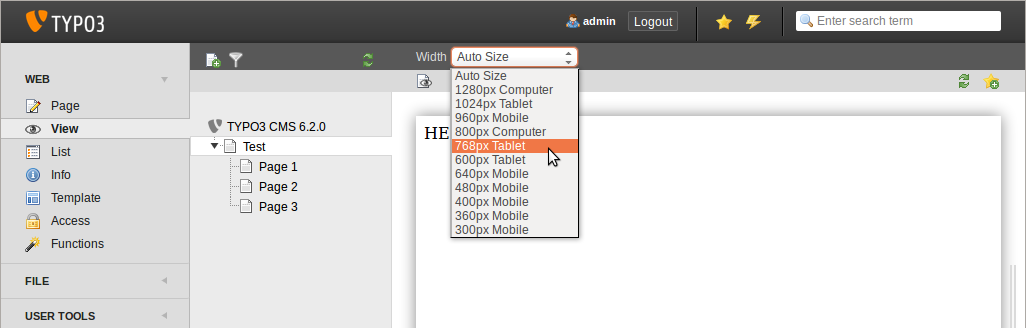
\includegraphics[width=0.95\linewidth]{Images/ResponsiveImages/ScreenSizeInPagePreview.png}
	\end{figure}

\end{frame}

% ------------------------------------------------------------------------------
% Customize Available Screen Sizes
% ------------------------------------------------------------------------------

\begin{frame}[fragile]
	\frametitle{Imágenes Responsivas}
	\framesubtitle{Personalizar Tamaños de Pantalla Disponibles}

	\begin{itemize}
		\item Los tamaños de pantalla son configurables vía PageTSconfig:

		\lstset{
			basicstyle=\fontsize{7}{9}\selectfont\ttfamily
		}

		\begin{lstlisting}
			mod.web_view.previewFrameWidths {
			  1780.label = <any LLL or string>
			  1780.height = 145
			}
		\end{lstlisting}

		\item El ancho se define por clave (aquí: 1780), la altura es opcional
		\item Pueden encontrarse tamaños predefinidos en el fichero:\newline
			\small\texttt{typo3/sysext/core/Configuration/DefaultConfiguration.php}\normalsize
		\item Pueden definirse etiquetas vía PageTSconfig:

		\begin{lstlisting}
			mod.web_view.previewFrameWidths {
			  1280.label = LLL:EXT:viewpage/Resources/Private/Language/locallang.xlf:computer
			  1024.label = LLL:EXT:viewpage/Resources/Private/Language/locallang.xlf:tablet
			}
		\end{lstlisting}

	\end{itemize}

\end{frame}

% ------------------------------------------------------------------------------
% Responsive Image Galleries
% ------------------------------------------------------------------------------

\begin{frame}[fragile]
	\frametitle{Imágenes Responsivas}
	\framesubtitle{Galerías de Imágenes Responsivas}

	\begin{itemize}
		\item Atributos adicionales para implementar galerías de imágenes responsivas
		\item "CSS styled content" expandido para conseguir esto
		\item Ejemplo: HTML5 (requiere \texttt{config.doctype = html5})\newline

			TYPO3 CMS < 6.2:

			\lstset{
				basicstyle=\fontsize{7}{9}\selectfont\ttfamily
			}

			\begin{lstlisting}
				<div class="csc-textpic-imagewrap">...</div>
			\end{lstlisting}

			TYPO3 CMS >= 6.2:

			\begin{lstlisting}
				<div class="csc-textpic-imagewrap"
				  data-csc-images="{register:imageCount}"
				  data-csc-cols="{field:imagecols}">...</div>
			\end{lstlisting}

	\end{itemize}

\end{frame}

% ------------------------------------------------------------------------------
% Responsive Image Rendering
% ------------------------------------------------------------------------------

\begin{frame}[fragile]
	\frametitle{Imágenes Responsivas}
	\framesubtitle{Renderizado de Imágenes Responsivas}

	\begin{itemize}
		\item cObject IMAGE renderiza la denominada "sourceCollection" para soportar varias dimensiones de pantalla
		\item Renderizado responsivo de imagen para cObjects "text/image" y "image" requiere de dos ajustes en el Editor de Constantes:

			\texttt{styles.content.imgtext.responsive}\newline
			\texttt{styles.content.imgtext.layoutKey}

		\item Opciones válidas ("listas para usar") son:

			\begin{itemize}
				\item \texttt{default}:	\tabto{2cm} por defecto tag \texttt{<img>}
				\item \texttt{srcset}:	\tabto{2cm} tag \texttt{<img>} con fuentes suplentes como srcset-attribute
				\item \texttt{picture}:	\tabto{2cm} tag \texttt{<picture>} con source-child-tags
				\item \texttt{data}:	\tabto{2cm} tag \texttt{<img>} con fuentes suplentes como data-attributes
			\end{itemize}

	\end{itemize}

\end{frame}

% ------------------------------------------------------------------------------
% Property: layoutKey
% ------------------------------------------------------------------------------

\begin{frame}[fragile]
	\frametitle{Imágenes Responsivas}
	\framesubtitle{Propiedad: layoutKey}

	\begin{itemize}
		\item \texttt{layoutKey} define el diseño del renderizado\newline
			(esto es el código HTML, usado para el tag \texttt{<img>})
		\item Cada opción muestra un único comportamiento para el renderizado HTML
		\item Opción \texttt{default} renderiza el tag \texttt{<img>} tradicionalmente\newline
			(debe usarse esto, si el frontend no es responsivo)
		\item Implementar un diseño responsivo requiere de diferentes dimensiones de imágenes para varias resoluciones y tamaños de pantalla
		\item Dependiendo del framework HTML, las capacidades del navegador y la librería JavaScript (para el realzamiento progresivo):

			\begin{itemize}
				\item Use una de las disposiciones predefinidas
				\item Defina su propia disposición personalizada
			\end{itemize}

	\end{itemize}

\end{frame}

% ------------------------------------------------------------------------------
% Property: layout
% ------------------------------------------------------------------------------

\begin{frame}[fragile]
	\frametitle{Imágenes Responsivas}
	\framesubtitle{Propiedad: layout}

			\lstset{
				basicstyle=\tiny\ttfamily
			}

			\begin{lstlisting}
				layoutKey = {$styles.content.imgtext.layoutKey}
				layout {
				  default {
				    element = <img src="###SRC###" width="###WIDTH###" height="###HEIGHT###" ###PARAMS###
				      ###ALTPARAMS### ###BORDER######SELFCLOSINGTAGSLASH###>
				  }
				  srcset {
				    element = <img src="###SRC###" srcset="###SOURCECOLLECTION###" ###PARAMS###
				      ###ALTPARAMS### ###SELFCLOSINGTAGSLASH###>
				    source = |*|###SRC### ###SRCSETCANDIDATE###,|*|###SRC### ###SRCSETCANDIDATE###
				  }
				  picture {
				    element = <picture>###SOURCECOLLECTION###<img src="###SRC###" ###PARAMS###
				      ###ALTPARAMS######SELFCLOSINGTAGSLASH###></picture>
				    source = <source src="###SRC###" media="###MEDIAQUERY###"###SELFCLOSINGTAGSLASH###>
				  }
				  data {
				    element = <img src="###SRC###" ###SOURCECOLLECTION### ###PARAMS###
				      ###ALTPARAMS######SELFCLOSINGTAGSLASH###>
				    source = data-###DATAKEY###="###SRC###"
				  }
				}
			\end{lstlisting}

\end{frame}

% ------------------------------------------------------------------------------
% Property: layout.[layoutKey].element
% ------------------------------------------------------------------------------

\begin{frame}[fragile]
	\frametitle{Imágenes Responsivas}
	\framesubtitle{Propiedad: layout.[layoutKey].element (1)}


	\begin{itemize}
			\item \lstinline!###SRC###!\newline
				URL para el atributo: \texttt{src}

			\item \lstinline!###WIDTH###!\newline
				Ancho de la imagen (en píxeles) para el atributo: \texttt{width}

			\item \lstinline!###HEIGHT###!\newline
				Altura de la imagen (en píxeles) para el atributo: \texttt{height}

			\item \lstinline!###PARAMS###!\newline
				Parámetros adicionales definidos en cObject IMAGE

			\item \lstinline!###ALTPARAMS###!\newline
				Parámetros adicionales alternativos definidos en cObject IMAGE

	\end{itemize}

\end{frame}

% ------------------------------------------------------------------------------
% Property: layout.[layoutKey].element
% ------------------------------------------------------------------------------

\begin{frame}[fragile]
	\frametitle{Imágenes Responsivas}
	\framesubtitle{Propiedad: layout.[layoutKey].element (2)}

		\begin{itemize}
			\item \lstinline!###BORDER###!\newline
				Borde (en píxeles) para el atributo: \texttt{border}

			\item \lstinline!###SELFCLOSINGTAGSLASH###!\newline
				Tag de cierre, p.ej. \texttt{<img ... />} vs. \texttt{<img ... >}\newline
				(depende de \texttt{config.xhtmlDoctype} o \texttt{config.doctype})

			\item \lstinline!###SOURCECOLLECTION###!\newline
				Fuentes de imagen adicionales, depende del uso de diseño web responsivo.
				Se definen valores exactos en la clave: \texttt{layout.[layoutKey].source}

	\end{itemize}

\end{frame}

% ------------------------------------------------------------------------------
% Property: sourceCollection.[dataKey]
% ------------------------------------------------------------------------------

\begin{frame}[fragile]
	\frametitle{Imágenes Responsivas}
	\framesubtitle{Propiedad: sourceCollection.[dataKey]}

	\begin{itemize}
		\item Por defecto sourceCollection de EXT:css\_styled\_content
		\item Es altamente recomendable escribir su propia sourceCollection

			\lstset{
				basicstyle=\tiny\ttfamily
			}

			\begin{lstlisting}
				sourceCollection {
				  small {
				    width = 200
				    srcsetCandidate = 600w
				    mediaQuery = (max-device-width: 600px)
				    dataKey = small
				  }
				  smallRetina {
				    if.directReturn = 1
				    width = 200
				    pixelDensity = 2
				    srcsetCandidate = 600w 2x
				    mediaQuery = (max-device-width: 600px) AND (min-resolution: 192dpi)
				    dataKey = smallRetina
				  }
				}
			\end{lstlisting}
	\end{itemize}

\end{frame}

% ------------------------------------------------------------------------------
% Further Resources (External Links)
% ------------------------------------------------------------------------------

\begin{frame}[fragile]
	\frametitle{Imágenes Responsivas}
	\framesubtitle{Más Recursos}

	\begin{itemize}
		\item Ejemplo de código que funciona en:\newline
			\small\url{http://wiki.typo3.org/Responsive_Image_Rendering}\normalsize

		\item Artículo de Sven Wolfermann en typo3.org:\newline
			\small\url{http://typo3.org/news/article/responsive-image-rendering-in-typo3-cms-62/}\normalsize

		\item Especificación W3C:\newline
			\small\url{http://www.w3.org/html/wg/drafts/srcset/w3c-srcset/}\newline
			\small\url{http://www.w3.org/TR/html-picture-element/}

		\item Borrador de Trabajo del "Grupo de Comunidad de Imagen Responsiva":\newline
			\small\url{http://responsiveimages.org}\normalsize

	\end{itemize}

\end{frame}

% ------------------------------------------------------------------------------

